\section{Evaluation}
\label{s:evaluation}


%1. Collect terms
%2. Query search results.
%3. Crawl data and get ground truth (how
%many).
%4. Train model and select parameters use 5-fold stratified cross validation
%~\cite{scikit-learn}.

In the above section ~\autoref{s:methodology}, we propose the SWM and explains
how it can be used to do cloaking detection (outlier detection). There are three
parameters to be learned, the upper bound of inconsistent coefficient in
clustering phase $T_{learn}$, the lower bound of inconsistent coefficient in the detection
phase $T_{detect}$, the fix parameter minimum radius $R_{detect}$. 
In order to measure cloaking in both SEO and SEM, we collects four candidate dataset
~\autoref{ss:dataset}. In this section,
we first describe the groundtruth obtained from $D_{hot, search}$ and $D_{spam,
search}$, then use it to train and test the performance of the proposed model.

\subsection{Groundtruth}

%We randomly sample 600 websites from the dataset, for 10 times. This results in
%5726 websites. We manually label them and \XXX{cloaking}, \XXX{not}, percentage
%for each is.
Similar to ~\cite{lin2009detection}, we start by remove duplicates (same simhash
from user view and Google view) from $D_{hot, search}$ and $D_{spam, search}$,
because these are not helpful for the algorithm training (designed to handle
dynamics of websites, non-changing websites are handled by default). Then we
manually label websites from $D_{hot, search}$ and $D_{spam, search}$ using
heuristics such as domain reputation ~\cite{wot} until we
have relatively large sample size for training. 
It is important to notice that, although the labeling process uses some url
reputation information (highly reputated domains are less likely to do cloaking),
it is not relevant to the algorithm, for algorithm only measures text difference
and layout difference of the original documents.
By conducting this massive
labeling process, we collect 1195 cloaking examples. In terms of normal websites, we randomly
select 5308 samples from non-cloaking dataset. The two parts, 6503 urls in
total, are combined as groundtruth $D_{g}$ for algorithm training and evaluation.
By applying feature extraction and simhash computation described in
~\autoref{ss:swm}, we have each url associated with its DOM simhash $S_{g, DOM}$ 
and text simhash $S_{g, text}$.

%\subsubsection{De-duplication}
%71116 urls
%
%62042 websites
%
%This results in \XXX{Some} links. Then we compare the text simhash and dom
%simhash, remove those which are exactly duplicate of one of the simhash observed
%by Google. After this step, we have \XXX{N} url left.
%
%For advertisements, after deduplication, there are 997 (score 60) urls remained.
%
%For search results, after deduplication 37155 urls, 35444 websites remained.



%We remove the failure websites and this results in 
%113242 urls, exact match, parameter different are counted.
%98390 sites, parameters ignored. Later we will use the latter parameter because
%it makes more sense.

%Step 1: Filter
%
%In order to get groundtruth, we follow a similar process employed in
%~\cite{lin2009detection}, we first filter the results and get rid of the highly reputated ones. We write a
%script to query the WOT API, and remove websites with combined score 80
%(which is a pretty high score) and the results are \XXX{N} urls after that.
%
%for advertisements, after filtering, there are 2279 (score 60) urls
%remained.\XXX{Problematic because I haven't merged them}
%
%for search results, after filtering, there are 90120 (60) urls remained.
%\XXX{Problematic because I haven't merged them}
%

%\subsubsection{Random Sample and Labeling}
%Then we randomly select 1000 urls from the dataset, and label them, after
%labeling, we found \XXX{N} cloaking sites and \XXX{M} dynamic websites.
%These are the groundtruth we used to label our data.


\subsection{Detection and Evaluation}
Regarding parameters to learn, $T_{learn}$ and $T_{detect}$ are parameters to
handle page dynamics, and $R_{detect}$ is a fix parameter to make system 
robust to consistent difference between spider and user copies, which doesnot
contribute to website modeling. Therefore, 
we first select optimal $T_{learn}$ and $T_{detect}$, and then present
system performance for different settings of $R_{detect}$.

\subsubsection{Selection of $T_{learn}$ and $T_{detect}$}
\label{sss:threshold}
Because $R_{detect}$ is a parameter to allow the system to handle consistent
difference between spider and user copies, therefore, we first set detect
$R_{detect}$ to be zero, and do five-fold stratified cross validation~\cite{scikit-learn}.
on with groundtruth $D_{g}$. In the learning phase,
our objective function is to first minimize the total number of errors in
classification $E = FP + FN, FP = \text{false positive}, FN = \text{false
negative}$, and
if $E$ is the same, minimize $d = T_{detect} - T_{learn}$.
This is reasonable because $d$ is the area that we cannot reject or accept. The smaller
the area, the more compact the learned model.
%The two objective
%function are widely used metrics in machine
%learning parameter selection \XXX{cite}.

By applying five-fold stratified cross validation on $S_{g, DOM}$ and $S_{g, text}$ and the described
objective function for optimal parameter selection, DOM simhash returned 
$T_{detect, DOM} = 1.8$ and $T_{learn, DOM} = 0.7$, and text simhash yields
$T_{detect, text} = 2.1$ and $T_{learn, text} = 0.7$.
% this is meaningless, i think
%
% majority is false positive.
% which yields to distance 1.1 at optimal (1318.4 learn error, 329 detect error), 

\subsubsection{Radius Selection $R_{detect}$}
Similarly, $R_{detect, text}$ and $R_{detect, DOM}$ are decided separately. In this section, we conduct
three experiments: cloaking detection using (1) DOM simhash (2) text simhash (3)
intersection DOM simhash and text simhash result.
Again, we use five-fold stratified cross validation and same objective function as in
~\autoref{sss:threshold} to learn and test $S_{g, DOM}$ and
$S_{g, text}$. The
optimal parameter for DOM simhash is $R_{detect, DOM} = 17$, text simhash is
$R_{detect, text} = 16$. ~\autoref{fig:roc} gives an illustration on
how False Positive Rate (FPR) and True Positive Rate (TPR) changes as
threshold for DOM and text changes. 
%If we consider significant difference in both text and dom as
%cloaking, the result is $R_{detect, dom} = 13$,
%$R_{detect, text} = 17$, and we get $FPR = 0.1\%, TPR = 94\%$.

Next, in order to show the combined result for different settings of $R_{detect,
dom}$, $R_{detect, text}$, we set $R_{detect, text}$ around its optimal value
and change $R_{detect, dom}$ as shown in ~\autoref{fig:roc}. It is obvious that
combining both DOM and text features improved the performance. 
The learned parameters are used in ~\autoref{s:measurement} to detect cloaking
on the four dataset, and since we want to capture as much cloaking as possible
for incentive study, we choose $R_{detect, text} = 15$ and $R_{detect, DOM} =
13$, which corresponds to 0.3\% FPR and 97.1\% TPR.

% you can also use the wonderful epsfig package...
\begin{figure}[t]
  \centering
  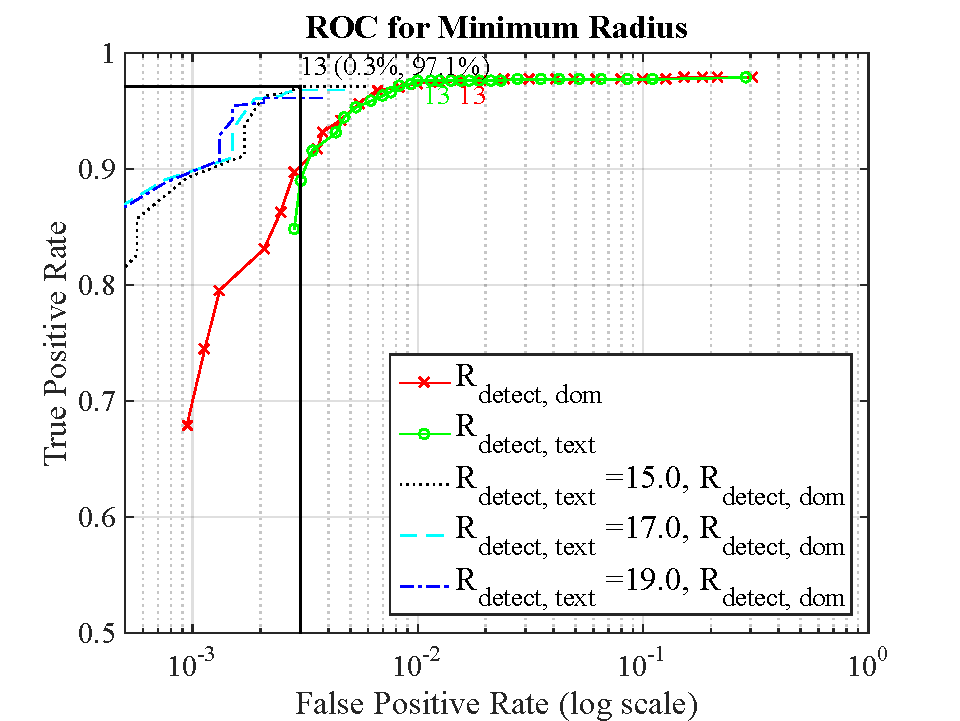
\includegraphics[width=.5\textwidth]{fig/roc}
  \caption{ROC for DOM, TEXT, DOM \& TEXT}
  \label{fig:roc}
\end{figure}

